\subsection{Data collection}

Which would you trust more: a poll where the people were randomly selected to take part or one where people searched out the poll to participate? Most polls reported in the media are of the first type while many polls on the internet are of the second type. Of the second, this is called a \term{convenience sample}, and these are generally not representative of the general population.

Ideally, a sample is selected randomly from the population that is representative. Individuals from every corner of the population at least have a chance of being included in the sample. This isn't always the case. If an internet poll, the only population that might be included are those of internet users.
\begin{center}
   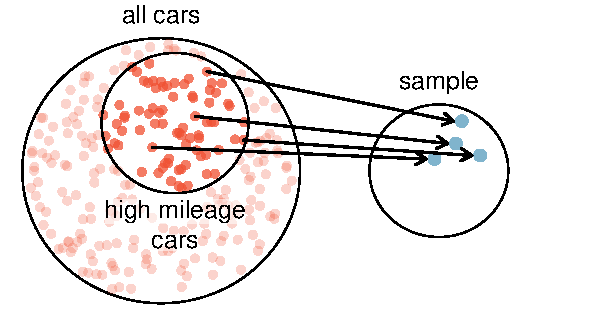
\includegraphics[height=1.6in]{ch1/popToSample/popToSubSample}
\end{center}
If the website had a political leaning, such as the liberal Huffington Post or the conservative CNS News' site, then an even smaller section of the population will be included that is rarely representative of the opinions of the population as a whole.
\begin{center}
   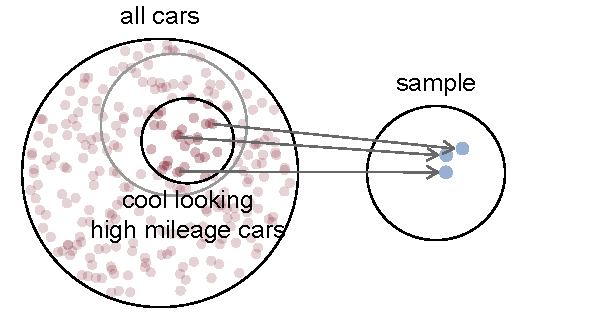
\includegraphics[height=1.6in]{ch1/popToSample/popToSubSubSample}
\end{center}
Convenience sampling usually invokes a \term{bias} into the data that can usually not be corrected.

Another difficulty in sampling is \term{self-selection bias}; individuals who participate must agree to do so. Granted, freedoms are certainly a good thing but the difficulties in sampling that arise from those freedoms are a nuisance when analyzing data, making interpretations of the data more difficult.

In addition to sampling the from the entire population, one of the most important components of sampling is selecting individuals from that population randomly. Another downfall of internet polls or any convenience sample is a \term{self-selection bias}; any individual in the sample actively choose to be in the sample.

Polls where the people polled are randomly selected from the population are more dependable for a specific reason: each person has an opportunity to be included in the sample. In a \term{simple random sample}, each person has an equal opportunity to be included. Most of the samples in this book are assumed to be simple random samples, and when this assumption is not necessarily reasonable it will be mentioned. For instance, it is not guaranteed that the possums are a simple random sample of possums in the sampled regions.
\begin{center}
   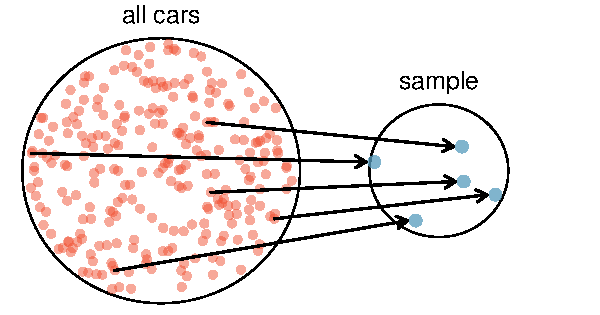
\includegraphics[height=1.6in]{ch1/popToSample/popToSample}
\end{center}
